% Options for packages loaded elsewhere
\PassOptionsToPackage{unicode}{hyperref}
\PassOptionsToPackage{hyphens}{url}
\PassOptionsToPackage{dvipsnames,svgnames,x11names}{xcolor}
%
\documentclass[
  letterpaper,
  DIV=11,
  numbers=noendperiod]{scrreprt}

\usepackage{amsmath,amssymb}
\usepackage{iftex}
\ifPDFTeX
  \usepackage[T1]{fontenc}
  \usepackage[utf8]{inputenc}
  \usepackage{textcomp} % provide euro and other symbols
\else % if luatex or xetex
  \usepackage{unicode-math}
  \defaultfontfeatures{Scale=MatchLowercase}
  \defaultfontfeatures[\rmfamily]{Ligatures=TeX,Scale=1}
\fi
\usepackage{lmodern}
\ifPDFTeX\else  
    % xetex/luatex font selection
\fi
% Use upquote if available, for straight quotes in verbatim environments
\IfFileExists{upquote.sty}{\usepackage{upquote}}{}
\IfFileExists{microtype.sty}{% use microtype if available
  \usepackage[]{microtype}
  \UseMicrotypeSet[protrusion]{basicmath} % disable protrusion for tt fonts
}{}
\makeatletter
\@ifundefined{KOMAClassName}{% if non-KOMA class
  \IfFileExists{parskip.sty}{%
    \usepackage{parskip}
  }{% else
    \setlength{\parindent}{0pt}
    \setlength{\parskip}{6pt plus 2pt minus 1pt}}
}{% if KOMA class
  \KOMAoptions{parskip=half}}
\makeatother
\usepackage{xcolor}
\setlength{\emergencystretch}{3em} % prevent overfull lines
\setcounter{secnumdepth}{5}
% Make \paragraph and \subparagraph free-standing
\makeatletter
\ifx\paragraph\undefined\else
  \let\oldparagraph\paragraph
  \renewcommand{\paragraph}{
    \@ifstar
      \xxxParagraphStar
      \xxxParagraphNoStar
  }
  \newcommand{\xxxParagraphStar}[1]{\oldparagraph*{#1}\mbox{}}
  \newcommand{\xxxParagraphNoStar}[1]{\oldparagraph{#1}\mbox{}}
\fi
\ifx\subparagraph\undefined\else
  \let\oldsubparagraph\subparagraph
  \renewcommand{\subparagraph}{
    \@ifstar
      \xxxSubParagraphStar
      \xxxSubParagraphNoStar
  }
  \newcommand{\xxxSubParagraphStar}[1]{\oldsubparagraph*{#1}\mbox{}}
  \newcommand{\xxxSubParagraphNoStar}[1]{\oldsubparagraph{#1}\mbox{}}
\fi
\makeatother


\providecommand{\tightlist}{%
  \setlength{\itemsep}{0pt}\setlength{\parskip}{0pt}}\usepackage{longtable,booktabs,array}
\usepackage{calc} % for calculating minipage widths
% Correct order of tables after \paragraph or \subparagraph
\usepackage{etoolbox}
\makeatletter
\patchcmd\longtable{\par}{\if@noskipsec\mbox{}\fi\par}{}{}
\makeatother
% Allow footnotes in longtable head/foot
\IfFileExists{footnotehyper.sty}{\usepackage{footnotehyper}}{\usepackage{footnote}}
\makesavenoteenv{longtable}
\usepackage{graphicx}
\makeatletter
\newsavebox\pandoc@box
\newcommand*\pandocbounded[1]{% scales image to fit in text height/width
  \sbox\pandoc@box{#1}%
  \Gscale@div\@tempa{\textheight}{\dimexpr\ht\pandoc@box+\dp\pandoc@box\relax}%
  \Gscale@div\@tempb{\linewidth}{\wd\pandoc@box}%
  \ifdim\@tempb\p@<\@tempa\p@\let\@tempa\@tempb\fi% select the smaller of both
  \ifdim\@tempa\p@<\p@\scalebox{\@tempa}{\usebox\pandoc@box}%
  \else\usebox{\pandoc@box}%
  \fi%
}
% Set default figure placement to htbp
\def\fps@figure{htbp}
\makeatother

\KOMAoption{captions}{tableheading}
\makeatletter
\@ifpackageloaded{tcolorbox}{}{\usepackage[skins,breakable]{tcolorbox}}
\@ifpackageloaded{fontawesome5}{}{\usepackage{fontawesome5}}
\definecolor{quarto-callout-color}{HTML}{909090}
\definecolor{quarto-callout-note-color}{HTML}{0758E5}
\definecolor{quarto-callout-important-color}{HTML}{CC1914}
\definecolor{quarto-callout-warning-color}{HTML}{EB9113}
\definecolor{quarto-callout-tip-color}{HTML}{00A047}
\definecolor{quarto-callout-caution-color}{HTML}{FC5300}
\definecolor{quarto-callout-color-frame}{HTML}{acacac}
\definecolor{quarto-callout-note-color-frame}{HTML}{4582ec}
\definecolor{quarto-callout-important-color-frame}{HTML}{d9534f}
\definecolor{quarto-callout-warning-color-frame}{HTML}{f0ad4e}
\definecolor{quarto-callout-tip-color-frame}{HTML}{02b875}
\definecolor{quarto-callout-caution-color-frame}{HTML}{fd7e14}
\makeatother
\makeatletter
\@ifpackageloaded{bookmark}{}{\usepackage{bookmark}}
\makeatother
\makeatletter
\@ifpackageloaded{caption}{}{\usepackage{caption}}
\AtBeginDocument{%
\ifdefined\contentsname
  \renewcommand*\contentsname{Table of contents}
\else
  \newcommand\contentsname{Table of contents}
\fi
\ifdefined\listfigurename
  \renewcommand*\listfigurename{List of Figures}
\else
  \newcommand\listfigurename{List of Figures}
\fi
\ifdefined\listtablename
  \renewcommand*\listtablename{List of Tables}
\else
  \newcommand\listtablename{List of Tables}
\fi
\ifdefined\figurename
  \renewcommand*\figurename{Figure}
\else
  \newcommand\figurename{Figure}
\fi
\ifdefined\tablename
  \renewcommand*\tablename{Table}
\else
  \newcommand\tablename{Table}
\fi
}
\@ifpackageloaded{float}{}{\usepackage{float}}
\floatstyle{ruled}
\@ifundefined{c@chapter}{\newfloat{codelisting}{h}{lop}}{\newfloat{codelisting}{h}{lop}[chapter]}
\floatname{codelisting}{Listing}
\newcommand*\listoflistings{\listof{codelisting}{List of Listings}}
\makeatother
\makeatletter
\makeatother
\makeatletter
\@ifpackageloaded{caption}{}{\usepackage{caption}}
\@ifpackageloaded{subcaption}{}{\usepackage{subcaption}}
\makeatother
<style>
div.callout-wpg.callout {
  border-left-color: #F1B300;
}
div.callout-wpg.callout-style-default > .callout-header {
  background-color: rgba(241, 179, 0, 0.13);
}
div.callout-wpg .callout-toggle::before {  background-image: url('data:image/svg+xml,<svg xmlns="http://www.w3.org/2000/svg" width="16" height="16" fill="rgb(33, 37, 41)" class="bi bi-chevron-down" viewBox="0 0 16 16"><path fill-rule="evenodd" d="M1.646 4.646a.5.5 0 0 1 .708 0L8 10.293l5.646-5.647a.5.5 0 0 1 .708.708l-6 6a.5.5 0 0 1-.708 0l-6-6a.5.5 0 0 1 0-.708z"/></svg>');}
div.callout-wpg.callout-style-default .callout-icon::before, div.callout-wpg.callout-titled .callout-icon::before {
  background-image: url('data:image/svg+xml,<svg xmlns="http://www.w3.org/2000/svg" width="16" height="16" fill="%23F1B300" class="bi bi-exclamation-triangle" viewBox="0 0 16 16"><path d="M7.938 2.016A.13.13 0 0 1 8.002 2a.13.13 0 0 1 .063.016.146.146 0 0 1 .054.057l6.857 11.667c.036.06.035.124.002.183a.163.163 0 0 1-.054.06.116.116 0 0 1-.066.017H1.146a.115.115 0 0 1-.066-.017.163.163 0 0 1-.054-.06.176.176 0 0 1 .002-.183L7.884 2.073a.147.147 0 0 1 .054-.057zm1.044-.45a1.13 1.13 0 0 0-1.96 0L.165 13.233c-.457.778.091 1.767.98 1.767h13.713c.889 0 1.438-.99.98-1.767L8.982 1.566z"/></svg>');
}
</style>
\makeatletter
\@ifpackageloaded{fontawesome6}{}{\usepackage{fontawesome6}}
\makeatother

\usepackage{bookmark}

\IfFileExists{xurl.sty}{\usepackage{xurl}}{} % add URL line breaks if available
\urlstyle{same} % disable monospaced font for URLs
\hypersetup{
  pdftitle={Idaho Wheat Production Guide},
  colorlinks=true,
  linkcolor={blue},
  filecolor={Maroon},
  citecolor={Blue},
  urlcolor={Blue},
  pdfcreator={LaTeX via pandoc}}


\title{Idaho Wheat Production Guide}
\author{}
\date{}

\begin{document}
\maketitle

\renewcommand*\contentsname{Table of contents}
{
\hypersetup{linkcolor=}
\setcounter{tocdepth}{2}
\tableofcontents
}

\bookmarksetup{startatroot}

\chapter*{Welcome}\label{welcome}
\addcontentsline{toc}{chapter}{Welcome}

\markboth{Welcome}{Welcome}

\begin{center}\rule{0.5\linewidth}{0.5pt}\end{center}

\begin{center}\rule{0.5\linewidth}{0.5pt}\end{center}

The Idaho Wheat Production Guide is a ``one-stop shop'' where Idaho
wheat producers can access the latest research results and production
recommendations from wheat researchers in Idaho and surrounding region.

The Idaho Wheat Production Guide is produced by the University of Idaho
with support from the Idaho Wheat Commission. Contributors include Idaho
and regional researchers.

\section*{How to use this guide}\label{how-to-use-this-guide}
\addcontentsline{toc}{section}{How to use this guide}

\markright{How to use this guide}

Browse topics in the sidebar, or use the search bar in the top right
corner of this page. Save, download and print articles, bulletins, and
guide sections individually, or \href{}{download the full Wheat
Production Guide} as a printable booklet.

\section*{Are we missing something?}\label{are-we-missing-something}
\addcontentsline{toc}{section}{Are we missing something?}

\markright{Are we missing something?}

\href{mailto:egalvin@uidaho.edu}{Submit requests} for articles, topics
or resources you'd like to see included in this guide.

\bookmarksetup{startatroot}

\chapter*{About the Project}\label{about-the-project}
\addcontentsline{toc}{chapter}{About the Project}

\markboth{About the Project}{About the Project}

There are various University of Idaho bulletins associated with
production of wheat in Idaho, and many were produced years ago by UI
researchers who have long retired. The University researchers currently
working in wheat production are located throughout the state, each with
their own websites and research projects specific to their area of
expertise.

With the many scattered resources and old bulletins that are hard to
find and access, there was not one UI cereals or wheat website that
could be used by producers to access the latest research results and
production recommendations. At the request of the Idaho Wheat
Commission, an accessible wheat publication coordinating information for
producers in one location online and in a printable bulletin or
production guide was needed to address this information gap.

Coordination of the available resources will also allow us to identify
gaps in the current research and prioritize funding to address those
gaps.

\section*{Contributors}\label{contributors}
\addcontentsline{toc}{section}{Contributors}

\markright{Contributors}

This guide is a project of the University of Idaho, with funding from
the Idaho Wheat Commission. Contributors include Idaho and regional
researchers.

\subsection*{People}\label{people}
\addcontentsline{toc}{subsection}{People}

\begin{itemize}
\tightlist
\item
  Dr.~Juliet M Marshall, Ext. Crop Mgmt. Specialist (SC and E Idaho)\\
\item
  Douglas Finkelnburg, Area Extension Educator, Cropping Systems (N
  Idaho)\\
\item
  Justin Hatch, Extension Educator, Caribou County\\
\item
  Dr.~Kurtis Schroeder, Moscow, Ext. Crop Mgmt. Specialist (N Idaho)\\
\item
  Dr.~Julia Piaskowski, CALS Director of Statistical Programs\\
\item
  Emily Galvin, Data Curation Technician, CALS Research Administration\\
\item
  Many others.
\end{itemize}

\subsection*{Funding Sources}\label{funding-sources}
\addcontentsline{toc}{subsection}{Funding Sources}

This project is financially supported by:

\begin{itemize}
\tightlist
\item
  \href{https://www.idahowheat.org/}{Idaho Wheat Commission}\\
\item
  \href{https://www.uidaho.edu/cals/idaho-agricultural-experiment-station}{Idaho
  Agricultural Experiment Station}
\end{itemize}

\section*{Contact}\label{contact}
\addcontentsline{toc}{section}{Contact}

\markright{Contact}

Please reach out if you have questions or would like to contribute to
the Guide!\\
\href{mailto:egalvin@uidaho.edu}{Emily Galvin}, Project Coordinator

\bookmarksetup{startatroot}

\chapter{Basic Recommendations and Quick
Facts}\label{basic-recommendations-and-quick-facts}

\subsection{Introduction}\label{introduction}

The unique quality characteristics of wheat protein lends itself as
essential to the production of leavened breads, while other classes of
wheat are used in various products such as cookies, pastries, noodles,
cakes and pancakes {[}@johnson1987{]}.

\subsubsection{Origin of wheat and environmental
adaptation}\label{origin-of-wheat-and-environmental-adaptation}

Wheat and other cereal grains were instrumental in the evolution of
human societies {[}@cropsa1992{]}. Several of the earliest known
civilizations in the Near East's fertile crescent co-evolved with modern
wheat. From the first collection and cultivation of cereals to modern
production, wheat has been used predominantly as a source of food and
less for feed and forage. Worldwide cultivation reflects both the
capacity for environmental adaptation and the reliance of humans on
wheat as a critical food source. Currently 20\% of the world
population's caloric and protein intake is based on wheat
{[}@erenstein2022{]}, with sustainable methods of production supporting
both food and economic stability.

\begin{figure}

\centering{

\pandocbounded{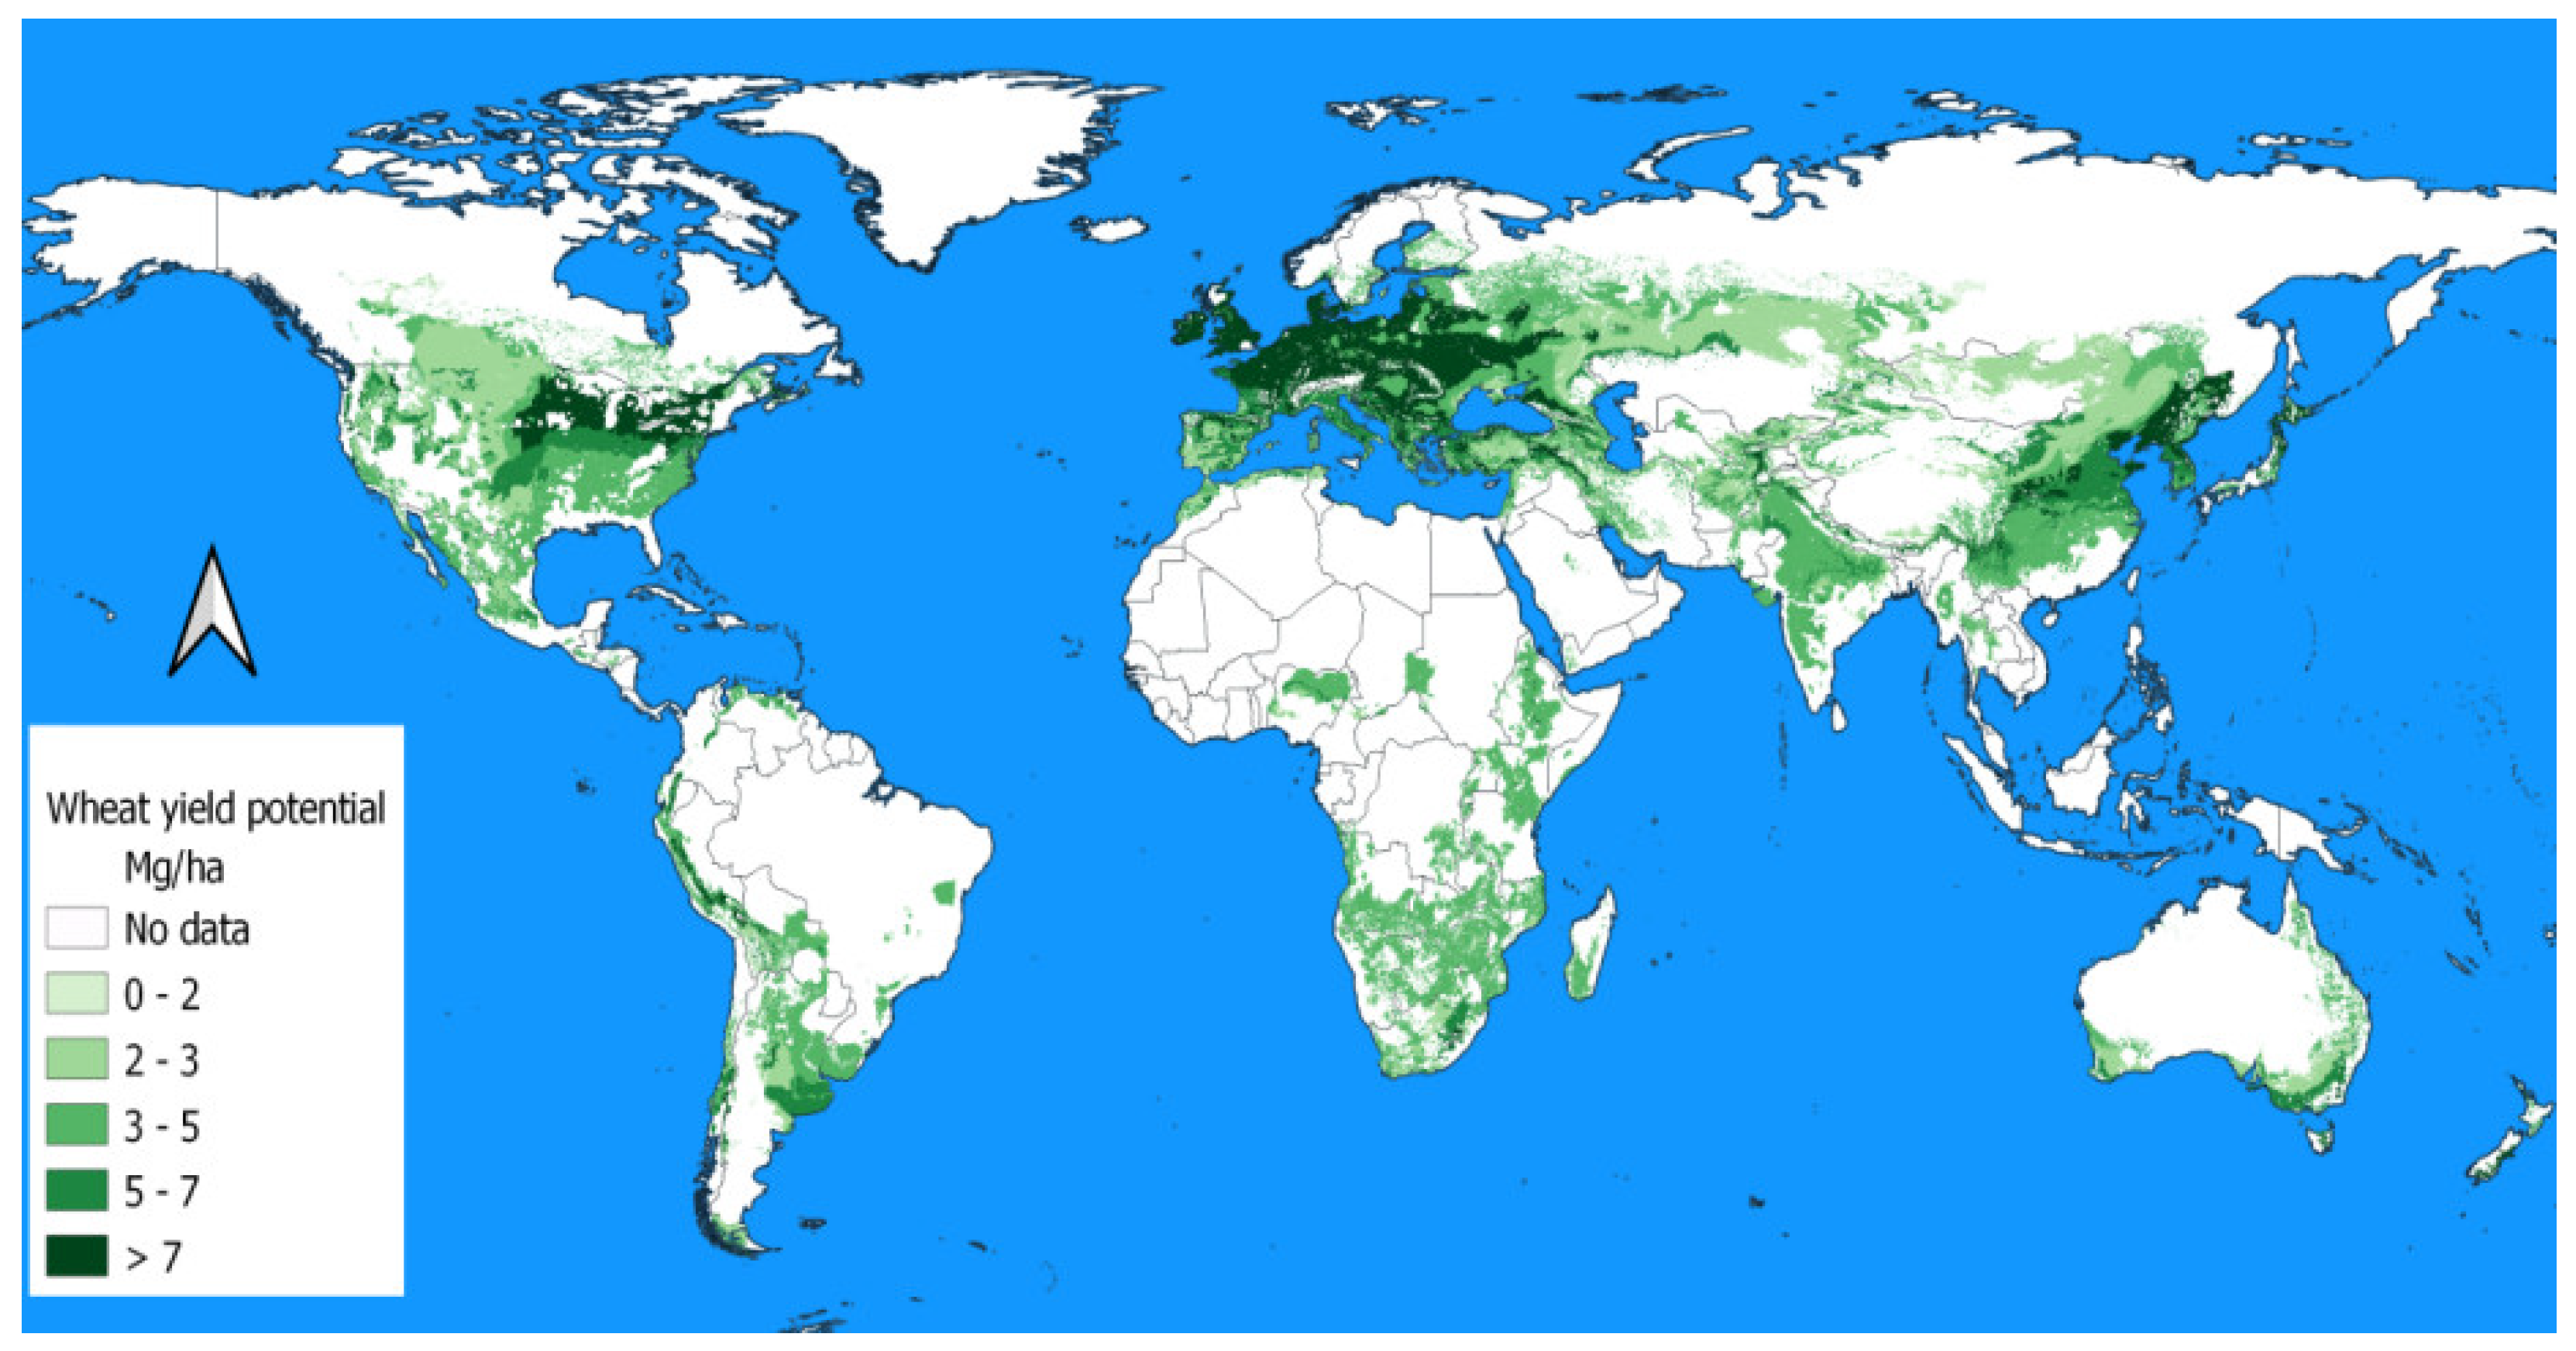
\includegraphics[keepaspectratio]{figs/1-1-global-wheat-production.png}}

}

\caption{\label{fig-global}World wheat production potential
{[}@halecki2022{]}.}

\end{figure}%

\subsubsection{US wheat cultivation}\label{us-wheat-cultivation}

Various regions in the US specialize in production of different classes
of wheat. Generally, regions specialize in the production of one or two
of the main market classes: soft red winter wheat, hard red winter
wheat, hard red spring wheat, hard white, soft white wheat (including
club wheats), and durum. The Central Plains states produce high protein
wheat for bread markets while lower protein soft red wheat is produced
in the eastern and southern regions east of the Mississippi. Development
of production systems depends on the market, the environment, the length
of the growing season and the dominant crop rotation. Unique to the PNW,
five market classes are produced across the region, requiring different
production practices and specialized grain handling.

\begin{figure}

\centering{

\pandocbounded{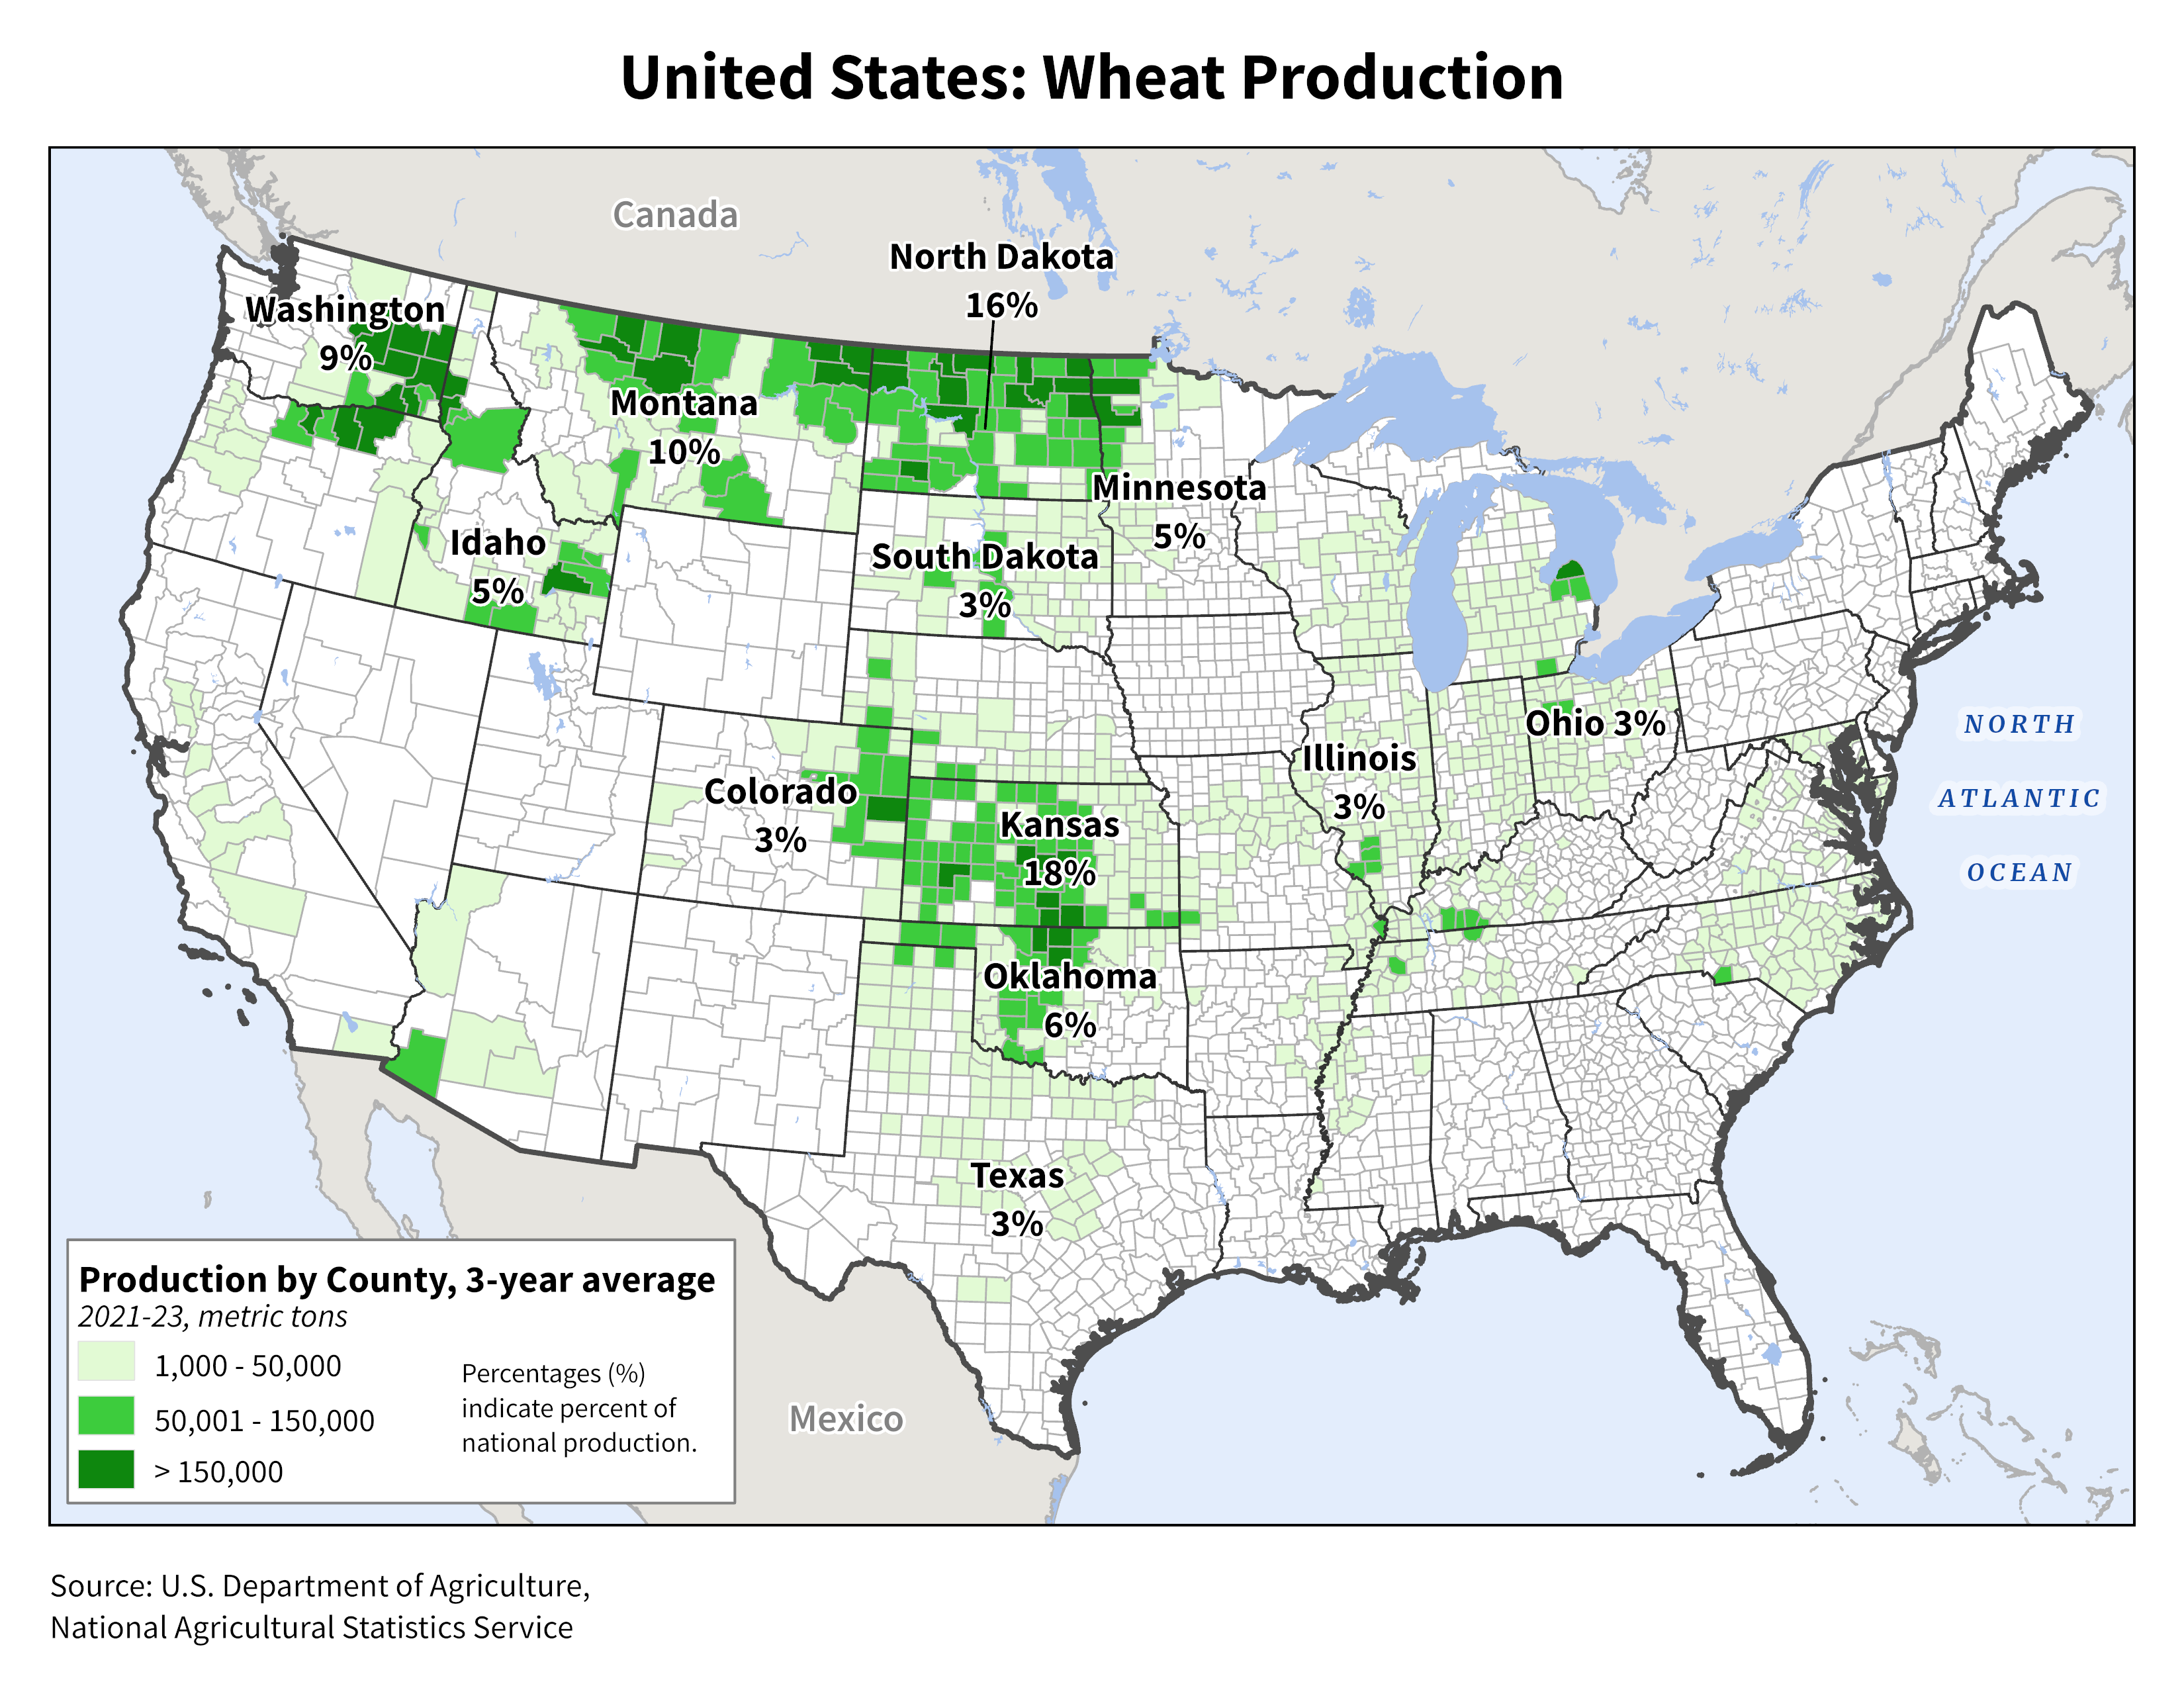
\includegraphics[keepaspectratio]{figs/1-2-us-wheat.png}}

}

\caption{\label{fig-us-wheat}Wheat production in the United States by
county, in metric tons. 3-year average, 2021-2023.}

\end{figure}%

\section{Idaho Wheat Quick Facts}\label{idaho-wheat-quick-facts}

\subsubsection{Statewide wheat production in Idaho,
2024}\label{tbl-idprod}

\begin{longtable}[]{@{}
  >{\raggedright\arraybackslash}p{(\linewidth - 6\tabcolsep) * \real{0.2500}}
  >{\centering\arraybackslash}p{(\linewidth - 6\tabcolsep) * \real{0.2500}}
  >{\centering\arraybackslash}p{(\linewidth - 6\tabcolsep) * \real{0.2500}}
  >{\centering\arraybackslash}p{(\linewidth - 6\tabcolsep) * \real{0.2500}}@{}}
\toprule\noalign{}
\begin{minipage}[b]{\linewidth}\raggedright
Habit
\end{minipage} & \begin{minipage}[b]{\linewidth}\centering
Harvested Area (acres)
\end{minipage} & \begin{minipage}[b]{\linewidth}\centering
Yield (bu/A)
\end{minipage} & \begin{minipage}[b]{\linewidth}\centering
Production (bu)\footnote{60 lb = 1 bu}
\end{minipage} \\
\midrule\noalign{}
\endhead
\bottomrule\noalign{}
\endlastfoot
Winter wheat & 700,000 & 89 & 62,300,000 \\
Spring wheat & 435,000 & 89 & 38,715,000 \\
\end{longtable}

\emph{Source:
\href{https://www.nass.usda.gov/Statistics_by_State/Idaho/index.php}{USDA
National Agricultural Statistics Service}}

\subsection{Southern Idaho Wheat
Factsheets}\label{southern-idaho-wheat-factsheets}

\bookmarksetup{startatroot}

\chapter{Wheat in Idaho -
Introduction}\label{wheat-in-idaho---introduction}

\pandocbounded{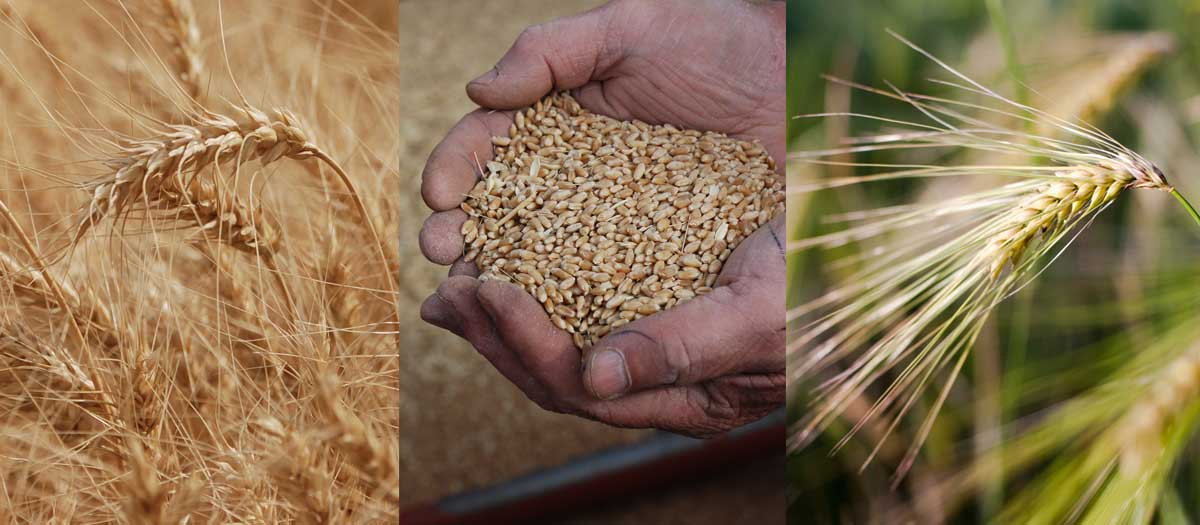
\includegraphics[keepaspectratio]{images/1200x525-cereals.jpg}}

Wheat is an important crop throughout the Pacific Northwest and the US.
Growers seed nearly 1.2 million acres every year, and yearly cash
receipts have averaged \$600 million in recent years. This places wheat
consistently in the top five for on-farm cash receipts of the crops in
Idaho. While wheat is produced across the region, production systems
vary greatly due to different climates, soils and availability of
irrigation. Wheat production systems in Idaho can be broken down into
three major areas: Northern Idaho rainfed production systems, Southern
Idaho Dryland production systems and Southern Idaho irrigated production
systems.

\subsection{Northern Idaho Rainfed Wheat Production
Systems}\label{northern-idaho-rainfed-wheat-production-systems}

Northern Idaho Rainfed Wheat Production Systems are characterized by
12-24 inches of annual precipitation on fields located between 1,000 --
4,000 feet above sea level. The northern Idaho ``Mediterranean Climate''
experiences typically mild winters and receives almost all its moisture
in the fall through spring months with typically extremely dry summer
months. Winter wheat is the most frequently planted crop in this region
and soft white wheat is the dominant market class grown. The majority of
soft white wheat bushels produced in this production region are exported
to Pacific Rim countries for use in noodles, crackers and sponge cakes.

\subsection{Southern Idaho Irrigated
Wheat}\label{southern-idaho-irrigated-wheat}

Key points:

\begin{itemize}
\tightlist
\item
  Wheat as a rotation crop with higher value row crops\\
\item
  Competition from malting barley and corn for dairies\\
\item
  Changes in the role of irrigated wheat in the past decade
\end{itemize}

\subsection{Southern Idaho Dryland
Wheat}\label{southern-idaho-dryland-wheat}

Winter wheat is an especially important crop in the dryland cropping
areas of southern Idaho. Approximately 125,000 acres are harvested
annually, producing over 4 million bushels of grain. Southern Idaho
dryland accounts for approximately 20 percent of the total state winter
wheat acreage and 10 percent of the total state wheat yield. Most
production in this environment is hard red winter wheat, with smaller
amounts of soft white winter and hard red spring wheat. Production of
hard white winter wheat is negligible at present but may increase in
future years.

In addition to the challenges of maintaining profitable farming
operations, wheat producers also face the challenge of conserving soil
and water resources in this area of rolling landscapes with high wind
and water erosion potential. High erosion potential, low crop residue
production, and generally low, sporadic precipitation make profitable
and sustainable cereal production challenging in this area. The goal of
every producer should be to obtain optimum yields that are affordable
for both short- and long-term considerations and that maximize the
efficient use of available land, management resources, and the
environment. This production guide brings together the best available
research information on management practices for economic and
environmentally sound production of wheat in Idaho.

\section{Agronomic zones}\label{agronomic-zones}

Learn more about agronomic zones:

\begin{itemize}
\tightlist
\item
  \href{https://extension.oregonstate.edu/sites/extd8/files/documents/pnw354.pdf}{Agronomic
  Zones of the Dryland Pacific Northwest - PNW Extension}\\
\item
  \href{https://pubs.extension.wsu.edu/product/advances-in-dryland-farming-in-the-inland-pacific-northwest-pnw697-reacch-handbook/}{Advances
  in Dryland Farming in the Inland Pacific Northwest - PNW Extension}\\
\end{itemize}

\section{Production, acreage, classes,
quality}\label{production-acreage-classes-quality}

\section{Markets -- domestic and
export}\label{markets-domestic-and-export}

\href{https://www.uswheat.org/market-information/}{US Wheat - Market
Information}

\bookmarksetup{startatroot}

\chapter{Growth and Development}\label{growth-and-development}

\textbf{\emph{intro/summary text}}

\section{Spring wheat}\label{spring-wheat}

\textbf{\emph{section text}}

Learn about the Zadoks growth staging system:\\
\href{https://extension.umn.edu/growing-small-grains/spring-wheat-growth-and-development-guide}{Spring
Wheat Growth and Development - UMN Extension}

\section{Winter wheat}\label{winter-wheat}

\textbf{\emph{section text}}

Learn about the stages of the Feekes Growth Scale:

\begin{figure}[H]

{\centering \pandocbounded{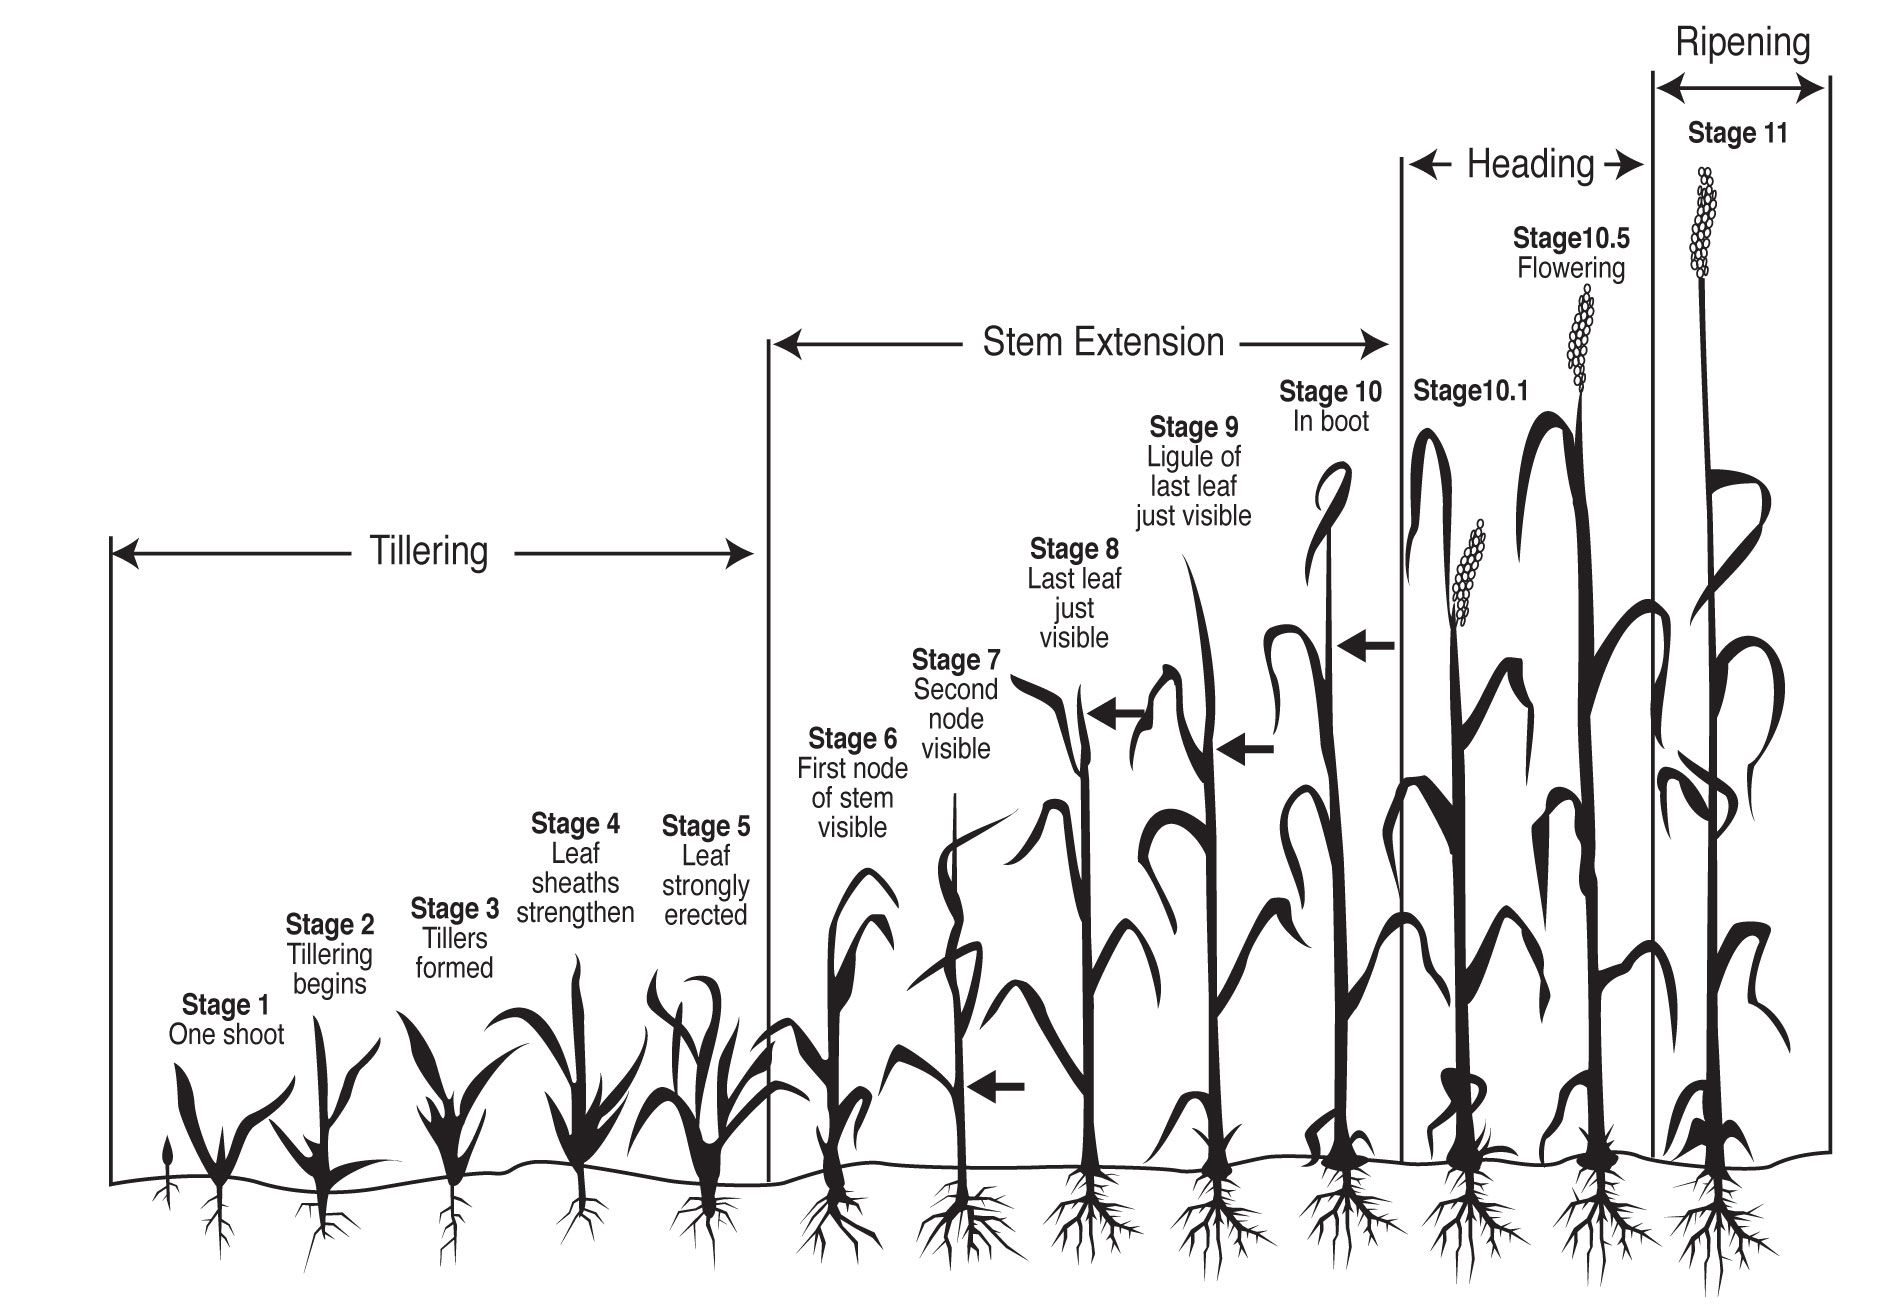
\includegraphics[keepaspectratio]{images/growth_stages.jpg}}

}

\caption{\emph{Image: Jerry Downs. Adapted from EC Large (1954), Plant
Pathology 3, pp128--129.}}

\end{figure}%

\href{https://ohioline.osu.edu/factsheet/agf-126}{Wheat Growth Stages
and Associated Management - Ohio Extension}

\href{https://bookstore.ksre.ksu.edu/pubs/MF3300.pdf}{Wheat Growth and
Development - KSU Extension}

Learn more about winter and spring growth stages:\\
\href{https://extension.sdstate.edu/sites/default/files/2020-03/S-0005-03-Wheat.pdf}{Winter
and Spring Wheat Growth Stages - SDSU Extension}

\bookmarksetup{startatroot}

\chapter{Wheat varieties and
breeding}\label{wheat-varieties-and-breeding}

\textbf{\emph{intro/summary text}}

\emph{Image: J Piaskowski}

\section{Key attributes for Idaho production
conditions}\label{key-attributes-for-idaho-production-conditions}

\textbf{\emph{section text}}

\section{Breeding -- public and private
programs}\label{breeding-public-and-private-programs}

\textbf{\emph{section text}}

\href{https://www.uidaho.edu/cals/aberdeen-research-and-extension-center/wheat-breeding}{Aberdeen
Wheat Breeding Program}\\
\href{https://breadlab.wsu.edu/research/wsu-breadlab-varieties/}{WSU
Breadlab}

\section{Herbicide resistant
varieties}\label{herbicide-resistant-varieties}

\textbf{\emph{section text}}

\section{Performance trials, supporting
data}\label{performance-trials-supporting-data}

\textbf{\emph{section text}}

\href{https://www.uidaho.edu/extension/cereals/north/variety-trials}{North
Idaho Cereals}\\
\href{https://www.uidaho.edu/extension/cereals/scseidaho/sgr}{South
Central \& Southeast Idaho Cereals}\\
\href{https://www.uidaho.edu/extension/cereals/southwest/varieties}{Southwest
Idaho Cereals}\\
\href{https://cropandsoil.oregonstate.edu/wheat/variety-trials}{Oregon
Cereals}\\
\href{https://smallgrains.wsu.edu/variety/archives/}{Eastern Washington
Cereals} \href{https://breadlab.wsu.edu/research/test-results/}{WSU
Breadlab}

\bookmarksetup{startatroot}

\chapter{Variety trial database}\label{variety-trial-database}

The Idaho Wheat Commission funded a statewide database of wheat variety
trials that expanded across the region to include Washington and Oregon,
and additional crops of barley, canola, and cool season legumes. The
University of Idaho in collaboration with Oregon State University and
Washington State University has combined and organized these data sets
into a set of tools collectively called ``\href{}{WAVE'' - the Western
Agricultural Variety Explorer}.

There are two major outputs:

\begin{itemize}
\item
  A \href{https://vartestdb.nkn.uidaho.edu/}{web interface} consisting
  of an online database of raw trial data.
\item
  Mobile apps for trial summaries.
\end{itemize}

These are different tools intended for distinct audiences.

\subsection{The Web Interface}\label{the-web-interface}

The online database contains raw data down to the plot level whenever
possible. This data can be searched by program (e.g.~Southeastern and
Southcentral Idaho), location, year, and market class. Anyone is welcome
to use this resource, but it is intended for researchers. There is
extensive trial metadata. Our goal was for every trial to include the
planting date, harvest date, plot number, and trial design, in addition
to year and location. When possible, we also captured exact
geocoordinates of each trial, soil test information, fertilizer and
other chemical applications, tillage regime, and planter type. We were
also able to capture additional information on row and range position of
each plot in the trial which enabled us to conduct spatial analysis of
each trial.

Extensive efforts were made to ensure that the data is correct and
consistent terminology is used. We defined acceptable limits for numeric
variables and standardized many categorical variables so that data sets
across programs could be combined. The
\href{https://vartestdb.nkn.uidaho.edu/user-guide}{user guide} provides
more details on how to access and use the database.

We have had over 2000 trials conducted across 70 locations over 20
years. Data this extensive can be used for many research applications;
understanding varietal changes over time, predicting performance of
trialed cultivars into a new environment that they have not previously
been evaluated, evaluating how timing of planting and harvesting has
changed over time, and other applications have helped us understand
wheat production across Pacific Northwest production zones and how we
can improve on that. The data here reflects the raw information used to
populate the information in the phone app.

\subsection{Mobile App}\label{mobile-app}

The target audience for the mobile app are producers and industry
representatives who want to look at final results from individual
variety trials. The three functions of the app are single trial,
multiple years, and cultivar explorer.

\begin{tcolorbox}[enhanced jigsaw, bottomrule=.15mm, opacityback=0, colback=white, left=2mm, titlerule=0mm, breakable, colframe=quarto-callout-color-frame, colbacktitle=quarto-callout-color!10!white, toprule=.15mm, rightrule=.15mm, coltitle=black, title={Single Trial Explorer}, leftrule=.75mm, toptitle=1mm, bottomtitle=1mm, arc=.35mm, opacitybacktitle=0.6]

This is for examining individual trials conducted within the last 5
years. There is a filter that can be used to drill down to the program,
market class, location, and year. Each trial was analyzed with a mixed
model where cultivar is a fixed effect and block is a random effect.
When possible, spatial covariate was included in the model to improve
the accuracy of the estimates and recover more reliable rankings between
the evaluated cultivars and candidate cultivars. Available trial
metadata is displayed along with information for key performance
indicators: yield, test weight, protein content, days to heading,
falling number, and plant height. This information is not always
available for all traits and trials. Data can be sorted by trait data,
and users can select which traits to display or plot.

\end{tcolorbox}

\begin{tcolorbox}[enhanced jigsaw, bottomrule=.15mm, opacityback=0, colback=white, left=2mm, titlerule=0mm, breakable, colframe=quarto-callout-color-frame, colbacktitle=quarto-callout-color!10!white, toprule=.15mm, rightrule=.15mm, coltitle=black, title={Single Location, Multi-Year Trial Explorer}, leftrule=.75mm, toptitle=1mm, bottomtitle=1mm, arc=.35mm, opacitybacktitle=0.6]

This data is for a single location over multiple years. Like in the
single trial tab, there is a filter to choose the program, market class
and location of trial to view. This data is also the product of a linear
mixed model, using the estimates from the single trial analyses.
Cultivar is a random effect, year is a fixed effect, and the estimates
are weighted by the reciprocal of their standard errors from single
trial analysis, so high precision results are weighted higher than lower
precision trials. The results from these analyses are presented in plots
and tables similar to what is shown in the single trial tab. The
analysis is conducted across the last 5 years, but only years selected
by the user will be shown.

\end{tcolorbox}

\begin{tcolorbox}[enhanced jigsaw, bottomrule=.15mm, opacityback=0, colback=white, left=2mm, titlerule=0mm, breakable, colframe=quarto-callout-color-frame, colbacktitle=quarto-callout-color!10!white, toprule=.15mm, rightrule=.15mm, coltitle=black, title={Cultivar Explorer}, leftrule=.75mm, toptitle=1mm, bottomtitle=1mm, arc=.35mm, opacitybacktitle=0.6]

This tab is for finding information for a specific cultivar. The results
shown in this tab are derived from the analyses of individual trials and
are limited to released cultivars only. Users must apply filters for
market class only, then can search on cultivar name. All trials where
the cultivar was tried will be shown in the filter that the user can
further narrow if they want. A small number of cultivars have been
trialed across a large number of locations and years; most cultivars
were trialed for a few years.

\end{tcolorbox}

The phone app is available in the
\href{https://apps.apple.com/us/app/u-of-i-wave/id6476321661}{Apple App
Store} and
\href{https://play.google.com/store/apps/details?id=com.uidaho.rcds.wave}{Google
Play Store}. We are working to build similar resources for barley. Our
homepage and long-term landing page for WAVE is
\url{https://www.westernagdata.org/}. Please check here for project
updates and links to the database instances and web apps.

\begin{tcolorbox}[enhanced jigsaw, toprule=.15mm, bottomrule=.15mm, opacityback=0, arc=.35mm, colback=white, left=2mm, rightrule=.15mm, leftrule=.75mm, breakable, colframe=quarto-callout-note-color-frame]
\begin{minipage}[t]{5.5mm}
\textcolor{quarto-callout-note-color}{\faInfo}
\end{minipage}%
\begin{minipage}[t]{\textwidth - 5.5mm}

\vspace{-3mm}\textbf{Note}\vspace{3mm}

We also previously hosted a web application for interactive trial
exploration. We are pursuing relaunching that and sunsetting the phone
apps.

\end{minipage}%
\end{tcolorbox}

\bookmarksetup{startatroot}

\chapter{Seed}\label{seed}

\textbf{\emph{intro/summary text}}

\section{Seed production, quality, and
assessment}\label{seed-production-quality-and-assessment}

\textbf{\emph{section text}}

\section{Certification and standards}\label{certification-and-standards}

\textbf{\emph{section text}}

Learn more about seed certification:\\
\href{https://cdn.prod.website-files.com/5c032b32fb1b863f50b40146/65f9a60f0a067bc2123b10a5_General\%20P\%26P\%20rev\%202024.pdf}{General
Seed Certification Policies and Procedures in Idaho}\\
\href{https://www.idahocrop.com/standards}{Idaho Grain Certification
Standards}

\section{PVP and title 5}\label{pvp-and-title-5}

\textbf{\emph{section text}}

Learn more about Plant Variety Protection through the USDA-AMS:
\href{https://www.ams.usda.gov/services/plant-variety-protection}{PVPO
Factsheet}

\bookmarksetup{startatroot}

\chapter{Planting}\label{planting}

\textbf{\emph{intro/summary text}}

\section{Seedbed preparation}\label{seedbed-preparation}

\textbf{\emph{section text}}

\section{Seeding dates, rates, depth,
spacing}\label{seeding-dates-rates-depth-spacing}

\textbf{\emph{section text}}

Resources:\\
\href{https://content-hub.uidaho.edu/api/public/content/62b0b1bc3bc1444b896fa312ca84bc10?v=1e2d120f}{Planting
Dates in Wheat Production for Southern Idaho}

\section{Equipment, calibration, and
monitoring}\label{equipment-calibration-and-monitoring}

\textbf{\emph{section text}}

\bookmarksetup{startatroot}

\chapter{Irrigation management}\label{irrigation-management}

\textbf{\emph{intro/summary text}}

\section{Crop water use and
evapotranspiration}\label{crop-water-use-and-evapotranspiration}

\textbf{\emph{section text}}

\section{Soil water-holding capacity}\label{soil-water-holding-capacity}

\textbf{\emph{section text}}

\section{Irrigation systems and
scheduling}\label{irrigation-systems-and-scheduling}

\textbf{\emph{section text}}

Resources:

\href{https://www.uidaho.edu/-/media/uidaho-responsive/files/extension/publications/bul/bul0833.pdf}{Estimating
Water Requirements of Hard Red Spring Wheat for Final Irrigation}

\bookmarksetup{startatroot}

\chapter{Nutrient management}\label{nutrient-management}

\textbf{\emph{intro/summary text}}

\section{Soil tests and
interpretations}\label{soil-tests-and-interpretations}

\textbf{\emph{section text}}

\section{Sap and tissue analyses}\label{sap-and-tissue-analyses}

\textbf{\emph{section text}}

\section{Calculator - rates / dates / yield
goals}\label{calculator---rates-dates-yield-goals}

\textbf{\emph{section text}}

\href{https://smallfarms.oregonstate.edu/calculator}{OSU Organic
Fertilizer and Cover Crop Calculators}

\section{Northern Idaho - N fertility; Macro-nutrients;
Micro-nutrients}\label{northern-idaho---n-fertility-macro-nutrients-micro-nutrients}

\textbf{\emph{section text}}

Resources:

\href{https://www.uidaho.edu/-/media/uidaho-responsive/files/extension/publications/cis/cis0453.pdf}{Northern
Idaho Fertilizer Guide: Winter Wheat}\\
\href{https://extension.oregonstate.edu/catalog/pub/pnw-631-phosphorus-fertilization-late-planted-winter-wheat-no-till-fallow}{Phosphorus
Fertilization of Late-Planted Winter Wheat in No-Till Fallow}\\
\href{https://www.uidaho.edu/-/media/UIdaho-Responsive/Files/Extension/publications/cis/cis1101.pdf}{Northern
Idaho Fertilizer Guide: Soft White Spring Wheat}\\
\href{https://objects.lib.uidaho.edu/uiext/uiext30490.pdf}{Northern
Idaho Fertilizer Guide: Spring Wheat}\\
\href{https://pubs.extension.wsu.edu/dryland-winter-wheat-eastern-washington-nutrient-management-guide}{Dryland
Winter Wheat: Eastern Washington Nutrient Management Guide}

\section{Southern Idaho irrigated - N fertility; Macro-nutrients;
Micro-nutrients}\label{southern-idaho-irrigated---n-fertility-macro-nutrients-micro-nutrients}

\textbf{\emph{section text}}

Resources:

\href{https://verso.uidaho.edu/esploro/outputs/newsletterArticle/Optimum-Nitrogen-Rates-for-Wheat-Depend/996749626401851}{Optimum
Nitrogen Rates for Wheat Depend on the Environmental and Field-Specific
Conditions}
\href{https://www.uidaho.edu/-/media/uidaho-responsive/files/extension/publications/cis/cis0373.pdf}{Southern
Idaho Fertilizer Guide: Irrigated Winter Wheat}\\
\href{https://idahodocs.contentdm.oclc.org/digital/collection/p16293coll6/id/78702}{Southern
Idaho Fertilizer Guide: Irrigated Spring Wheat}

\section{Southern Idaho dryland - N fertility; Macro-nutrients;
Micro-nutrients}\label{southern-idaho-dryland---n-fertility-macro-nutrients-micro-nutrients}

\textbf{\emph{section text}}

Resources:\\
\href{https://objects.lib.uidaho.edu/uiext/uiext30376.pdf}{Idaho
Fertilizer Guide - Dryland Wheat Production in SE Idaho and N. Utah}

\section{PNW fertilizer guides - wheat classes and cropping
systems}\label{pnw-fertilizer-guides---wheat-classes-and-cropping-systems}

\textbf{\emph{section text}}

\subsubsection{Nitrogen and Protein Management
Guides:}\label{nitrogen-and-protein-management-guides}

\href{https://s3-us-west-2.amazonaws.com/smallgrains.wsu.edu/uploads/2019/03/Hard-Red-Spring-Wheat-Nitrogen-and-Protein-Brief-from-the-WA-Grain-Commission.pdf}{Hard
Red Spring Wheat Nitrogen and Protein Management Guide}\\
\href{https://wpcdn.web.wsu.edu/cahnrs/uploads/sites/16/Hard-Red-Winter-Wheat-Nitrogen-and-Protein-Brief-from-WA-Grain-Commission-2.pdf}{Hard
Red Winter Wheat Nitrogen and Protein Management Guide}

\href{https://wpcdn.web.wsu.edu/cahnrs/uploads/sites/16/Hard-White-Spring-Wheat-Nitrogen-and-Protein-Brief-from-the-WA-Grain-Commission-1.pdf}{Hard
White Spring Wheat Nitrogen and Protein Management Guide}

\subsubsection{Winter Wheat in Continuous and Summer Fallow Cropping
Systems - Fertilizer Guides (low, intermediate, and high precipitation
zones)}\label{winter-wheat-in-continuous-and-summer-fallow-cropping-systems---fertilizer-guides-low-intermediate-and-high-precipitation-zones}

\href{https://extension.oregonstate.edu/catalog/pub/fg-81-winter-wheat-spring-grains-continuous-cropping-systems-low-precipitation-zone}{Winter
Wheat and Spring Grains in Continuous Cropping Systems (Low
Precipitation Zone)}\\
\href{https://extension.oregonstate.edu/catalog/pub/fg-80-winter-wheat-summer-fallow-systems-low-precipitation-zone-fertilizer-guide}{Winter
Wheat in Summer-Fallow Systems (Low Precipitation Zone)}\\
\href{https://extension.oregonstate.edu/catalog/pub/fg-84-winter-wheat-continuous-cropping-systems-high-precipitation-zone-fertilizer-guide}{Winter
Wheat in Continuous Cropping Systems (High Precipitation Zone)}\\
\href{https://extension.oregonstate.edu/catalog/pub/fg-83-winter-wheat-continuous-cropping-systems-intermediate-precipitation-zone}{Winter
Wheat in Continuous Cropping Systems (Intermediate Precipitation
Zone)}\\
\href{https://extension.oregonstate.edu/catalog/pub/fg-82-winter-wheat-summer-fallow-systems-intermediate-precipitation-zone-fertilizer}{Winter
Wheat in Summer-Fallow Systems (Intermediate Precipitation Zone}

\section{Cover crops}\label{cover-crops}

\textbf{\emph{section text}}

\href{https://extension.oregonstate.edu/catalog/pub/pnw-636-estimating-plant-available-nitrogen-release-cover-crops}{Estimating
Plant-Available Nitrogen Release from Cover Crops}

\section{Biosolids}\label{biosolids}

\textbf{\emph{section text}}

Learn more:\\
\href{https://extension.oregonstate.edu/catalog/pub/pnw-508-fertilizing-biosolids}{Fertilizing
with Biosolids}

\section{Liming for acid soils}\label{liming-for-acid-soils}

\textbf{\emph{section text}}

Learn more:
\href{https://pubs.extension.wsu.edu/agriculture-lime-and-liming-part-1-introduction-to-agricultural-lime-and-liming-soil-acidification-series}{Agricultural
Lime and Liming (Parts 1-3)}\\
\href{https://pubs.extension.wsu.edu/acid-soils-how-do-they-interact-with-root-diseases-soil-acidification-series}{Acid
Soils: How do they Interact with Soil Disease}

\section{Impact on end-use quality}\label{impact-on-end-use-quality}

\textbf{\emph{section text}}

Resources:\\
\href{https://www.uidaho.edu/extension/publications/bul/bul957}{Irrigation
and Nitrogen Fertilization Affect End-Use Quality of Spring Wheat of
Three Market Classes}

\bookmarksetup{startatroot}

\chapter{Weed control}\label{weed-control}

\textbf{\emph{intro/summary text}}

Resources:\\
\href{https://pnwhandbooks.org/weed}{Weed Management Handbook}

\section{Cultural practices}\label{cultural-practices}

\textbf{\emph{section text}}

\section{Chemicals}\label{chemicals}

\textbf{\emph{section text}}

\section{Groups, interactions,
carryover}\label{groups-interactions-carryover}

\textbf{\emph{section text}}

Resources:\\
\href{https://extension.okstate.edu/fact-sheets/print-publications/pss/herbicide-how-to-understanding-herbicide-mode-of-action-pss-2778.pdf}{Understanding
Herbicide Mode of Action}

\href{https://wssa.net/wp-content/uploads/WSSA-Mechanism-of-Action.pdf}{Summary
of Herbicide Mechanism of Action According to the Weed Science Society
of America}

\section{Labels and recommendations}\label{labels-and-recommendations}

\textbf{\emph{section text}}

\section{Herbicide resistance}\label{herbicide-resistance}

\textbf{\emph{section text}}

\section{Chemical rotations, management
strategies}\label{chemical-rotations-management-strategies}

\textbf{\emph{section text}}

\bookmarksetup{startatroot}

\chapter{Diseases and disease
management}\label{diseases-and-disease-management}

\textbf{\emph{intro/summary text}}

\section{Foliar diseases}\label{foliar-diseases}

\textbf{\emph{section text}}

\section{Spike and seed-borne
diseases}\label{spike-and-seed-borne-diseases}

\textbf{\emph{section text}}

Learn more:\\
\href{https://objects.lib.uidaho.edu/uiext/uiext30078.pdf}{Seedborne
Diseases of Cereals}

\section{Soil-borne diseases}\label{soil-borne-diseases}

\textbf{\emph{section text}}

\bookmarksetup{startatroot}

\chapter{Insect pests and control}\label{insect-pests-and-control}

\textbf{\emph{intro/summary text}}

Learn more:\\
\href{https://pnwhandbooks.org/insect}{Insect Management Handbook}

\section{Integrated pest management}\label{integrated-pest-management}

\textbf{\emph{section text}}

\section{Aphids}\label{aphids}

\textbf{\emph{section text}}

\section{Wireworm}\label{wireworm}

\textbf{\emph{section text}}

\section{Hessian fly}\label{hessian-fly}

\textbf{\emph{section text}}

Learn more:\\
\href{https://pubs.extension.wsu.edu/fs331e-hessian-fly-management-in-wheat}{Hessian
Fly Management in Wheat}

\section{Nematodes}\label{nematodes}

\textbf{\emph{section text}}

Learn more:\\
\href{https://extension.oregonstate.edu/catalog/pub/pnw-620-cereal-cyst-nematode}{Cereal
Cyst Nematodes: Biology and Management in Pacific Northwest Wheat,
Barley, and Oat Crops}

\bookmarksetup{startatroot}

\chapter{Nematodes}\label{nematodes-1}

\begin{figure}

\centering{

\href{https://pnwhandbooks.org/plantdisease/pathogen-articles/common/nematodes}{\pandocbounded{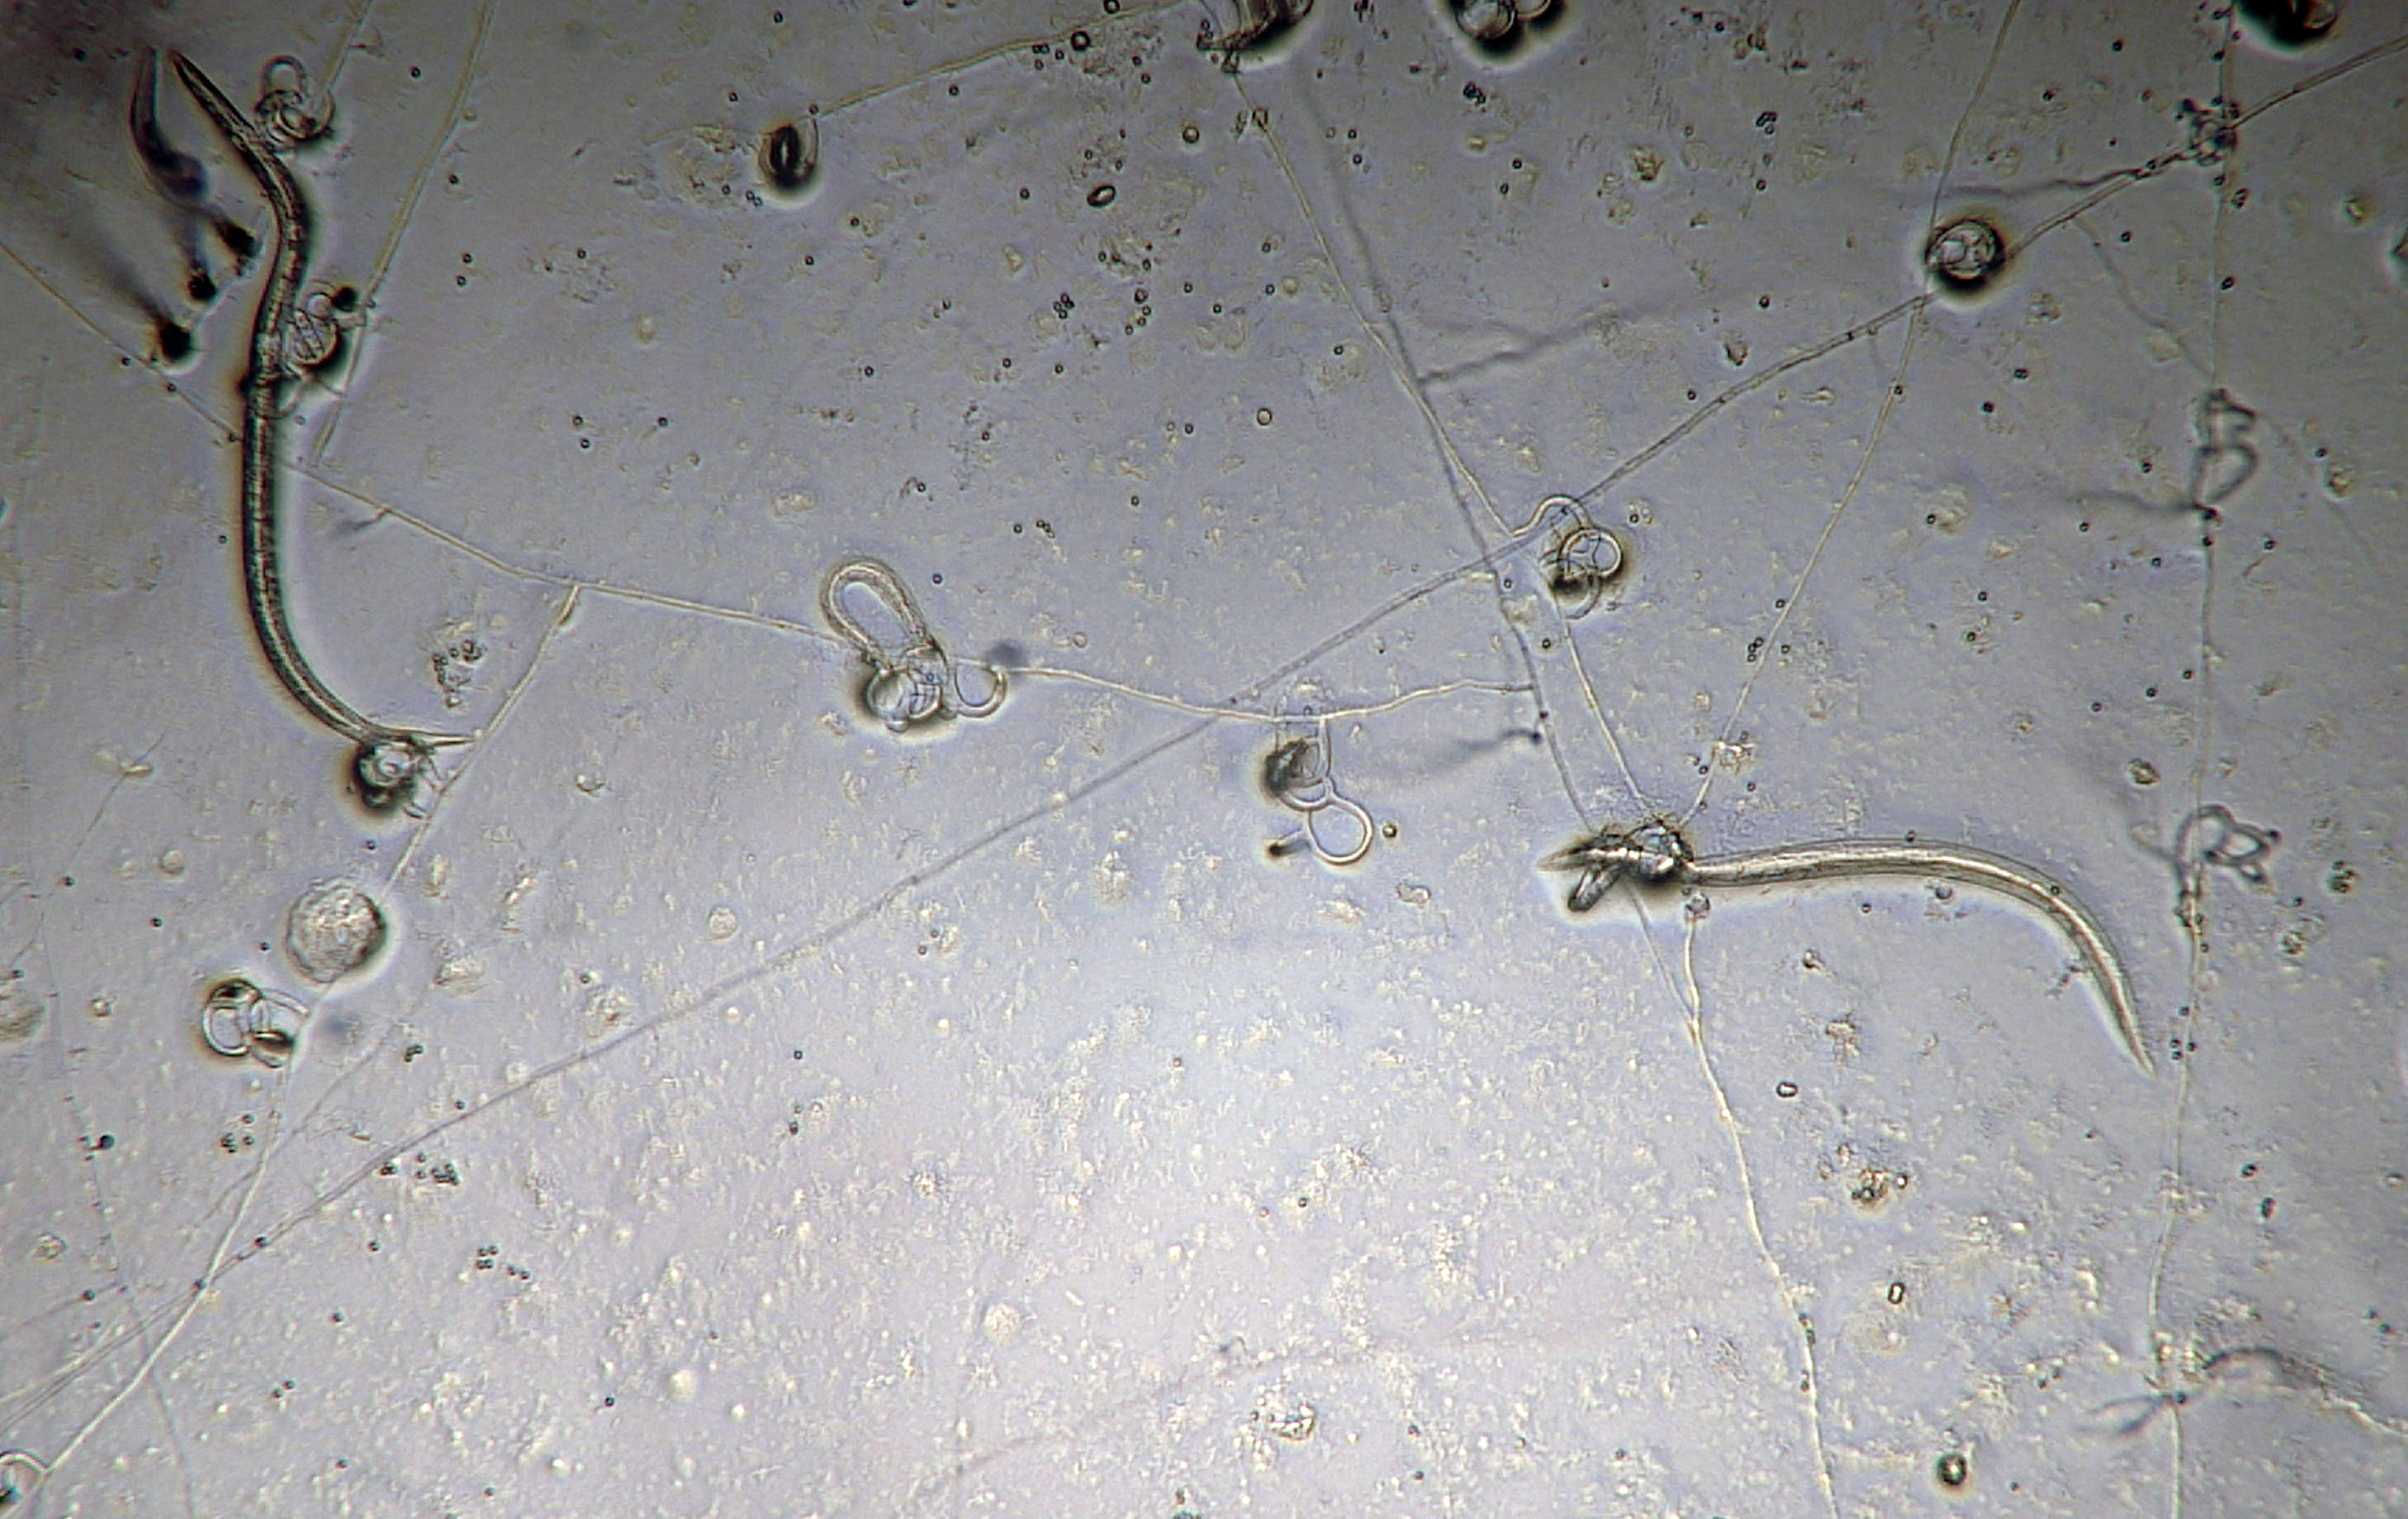
\includegraphics[keepaspectratio]{figs/nematode-trapping-fungus.jpg}}}

}

\caption{\label{fig-nema1}Nematode trapping fungus. OSU Plant Clinic,
2020.}

\end{figure}%

Further reading:\\
\href{https://extension.oregonstate.edu/catalog/pub/pnw-620-cereal-cyst-nematodes}{Cereal
Cyst Nematodes: Biology and Management in Pacific Northwest Wheat,
Barley, and Oat Crops}\\
\href{https://pnwhandbooks.org/plantdisease/pathogen-articles/common/nematodes}{PNW
Disease Management Handbook - Pathogen Articles - Nematodes}

\bookmarksetup{startatroot}

\chapter{Drones and UAV}\label{drones-and-uav}

\textbf{\emph{intro/summary text}}

\section{Applications and
calibrations}\label{applications-and-calibrations}

\textbf{\emph{section text}}

\bookmarksetup{startatroot}

\chapter{Harvest and storage}\label{harvest-and-storage}

\emph{Image: J Piaskowski}

\section{Summary}\label{summary}

This chapter emphasizes that maximizing wheat yield and quality requires
careful harvest timing, precise combine adjustment, and attentive
storage management. Harvest should occur before shattering from dry
weather or sprouting from rain, with grain at or below 12--12.5\%
moisture for safe storage; wetter grain, especially seed wheat, must be
dried promptly at temperatures below 110°F.

Combine settings for cylinder speed, concave clearance, fan speed, reel
speed, and ground speed should be fine-tuned in the field to minimize
losses from shattering, header inefficiency, leakage, and poor
separation, while managing heavy straw to avoid plugging and traction
hazards. Loss-measurement techniques help diagnose issues, and
specialized headers or reels can improve efficiency in lodged crops. In
storage, grain should be kept dry, cool (ideally below 50°F), and
insect-free, with clean bins, regular inspections, and aeration to
prevent heat and moisture migration that can cause spoilage, ensuring
that field grains are preserved until the wheat leaves storage.

\section{Harvesting}\label{harvesting}

Proper adjustment and operation of the combine reduces harvest losses.
Adjust the combine initially to specifications provided by the
manufacturer and field check for grain loss out of the back of the
combine. Depending on variety, approximately 16 to 20 kernels per square
foot on the ground represents a one bushel per acre loss. Adjust air
speed to separate chaff from grain without blowing grain out the back of
the combine. On cylinder-type combines, adjust cylinder speed and
concave clearance to thresh grain free without cracking. Periodic field
checks should be made during harvest to adjust for changing moisture
content of the straw and grain.

Wheat yield and volume of wheat straw is highly variable depending on
production system and growing environment. High-yielding spring wheat
varieties under irrigation can produce as much or more straw as
high-yielding dryland winter wheat, or as much as 5-7 tons of straw per
acre. The key to efficient harvest is controlling the amount of material
entering the cylinder for best grain separation and to avoid plugging.

\begin{tcolorbox}[enhanced jigsaw, bottomrule=.15mm, opacityback=0, colback=white, left=2mm, titlerule=0mm, breakable, colframe=quarto-callout-tip-color-frame, colbacktitle=quarto-callout-tip-color!10!white, toprule=.15mm, rightrule=.15mm, coltitle=black, title=\textcolor{quarto-callout-tip-color}{\faLightbulb}\hspace{0.5em}{Harvest Safety Tip}, leftrule=.75mm, toptitle=1mm, bottomtitle=1mm, arc=.35mm, opacitybacktitle=0.6]

Heavy straw residue can reduce equipment traction, especially on slopes.
Operators should identify areas where footing or control may be
compromised and adjust their approach to maintain safe working
conditions for themselves and the entire harvest crew.

\end{tcolorbox}

Management of a wheat crop for optimum health and production potential
must continue through harvest. There are several factors to consider
both during and after wheat harvest.

\section{Moisture Content}\label{moisture-content}

Moisture content is critical in preventing preharvest and postharvest
losses. To minimize preharvest losses, winter wheat must be harvested
before wind causes shattering under dry conditions or rain causes
sprouting in the head. The grain must be dry enough for safe storage,
preferably less than 12 to 12.5 percent moisture by weight. If moisture
content is higher than this, the grain must be dried prior to storage.
The general recommendation is to thresh at moistures not greater than 20
percent and to dry with air not exceeding 110°F (43°C), especially if
the wheat is to be used for seed, since higher temperatures can damage
germination.

\section{Combine Settings}\label{combine-settings}

Combines must be properly adjusted to minimize combine harvest losses
and to avoid cracking the grain, which invites greater damage from
storage molds and insects. Grain left on the ground, either because of
shattering or improper combine adjustments, represents grain that cannot
be sold, as well as a source of future volunteer plants to host diseases
and insects. Straw and chaff must be spread as uniformly as possible to
reduce problems in planting and performance of the following crop (see
Section~\ref{sec-management-considerations-for-conservation-tillage-systems}:
Management considerations for conservation tillage systems).

\section{Minimizing Losses from Shattering and
Sprouting}\label{minimizing-losses-from-shattering-and-sprouting}

The first step in minimizing losses from shattering and sprout damge is
to choose the appropriate variety of wheat for your area. Harvesting at
the ideal time and moisture content can reduce shattering and sprouting,
but this is often beyond the grower's control. Wheat can be harvested at
a moisture content higher than what is recommended, but this grain will
have to be dried before or immediately after it is placed in the bin. A
second option for dealing with wet wheat is swathing and allowing it to
dry in windrows on the stubble. Once the grain has reached the
maximum-weight phase of grain fill (see growth and development section),
the wheat can be swathed with no loss of yield. The grain is at
physiological maturity by this stage, but the plant is still alive and
has considerable moisture in the straw as well as in the grain. Swathing
speeds the drying process for the plant and grain.

\section{Minimizing Cracking and Combine
Losses}\label{minimizing-cracking-and-combine-losses}

Final combine adjustments to minimize cracking and combine losses must
be made in the field, several times each day and in each new field. The
tendency for kernels to crack or thresh out varies by day and even by
time of day, depending on the moisture content of the grain and straw.
Threshability of the grain also varies by wheat variety and by weed
population. Late-season green weeds may require swathing or a preharvest
burndown herbicide.

Critical adjustments on the combine include cylinder speed, fan speed,
reel speed, and ground speed. The cylinder speed and concave clearance
should thresh but not crack the grain. The fan speed should be adjusted
to blow out chaff but not grain. Avoid header losses (broken heads) by
setting the reel speed and cutting height to leave as much standing
stubble as possible. Adjust ground speed to set the rate of straw feed
to the straw walkers to optimize harvest efficiency. Initial adjustments
should be made as close to the manufacturer's operator manual as
possible, but final adjustments should be based on the actual field
performance of the combine.

Growers can accurately measure and monitor combine losses, including
shattering, header losses, leakage from the combine, and losses out the
rear of the combine, by following a few simple steps. With the straw
spreader disengaged, harvest a short strip of typical grain, then stop
and let the combine clean out. Mark the rear of the header (position B
in Figure 1) and in front of the rear wheels of the combine (position C
in Figure~\ref{fig-combine-15-1}), then back the combine to expose this
strip. The actual losses and reason for these losses can be estimated by
the location and the amount of grain on the ground.

\begin{figure}

\centering{

\pandocbounded{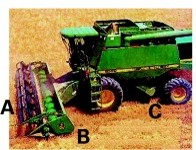
\includegraphics[keepaspectratio]{figs/combine-positions.jpg}}

}

\caption{\label{fig-combine-15-1}Combine positions used to determine
types of harvest losses.}

\end{figure}%

\subsection{Steps to Distinguish Header Losses from
Shattering}\label{steps-to-distinguish-header-losses-from-shattering}

\textbf{1. Identify Two Locations:}\\
- Position A: Standing grain --- used to measure shatter loss only.\\
- Position B: Recently harvested grain --- used to measure shatter loss
plus header loss.\\
\textbf{2. Mark Sampling Areas:}\\
- At each position, mark at least five one-foot-square areas.\\
- Ensure the sampling areas at Position B are uniformly spaced across
the header swath.\\
\textbf{3. Collect Data at Each Area:}\\
- Count the number of loose kernels on the ground.\\
- Count the number of broken heads on the ground.\\
\textbf{4. Calculate Averages:}\\
- For each position (A and B), calculate the average number of kernels
and broken heads per square foot.\\
\textbf{5. Determine Header Loss:}\\
- Subtract the average values at Position A (shatter loss) from the
average values at Position B (total loss).\\
- The difference represents the header loss.

\bookmarksetup{startatroot}

\chapter{Cropping systems}\label{cropping-systems}

\textbf{\emph{intro/summary text}}

\section{Rotations, interactions, and management
issues}\label{rotations-interactions-and-management-issues}

\textbf{\emph{section text}}

\section{Organic production}\label{organic-production}

\textbf{\emph{section text}}

Learn more:\\
\href{https://pubs.extension.wsu.edu/organic-small-grain-production-in-the-inland-pacific-northwest-a-collection-of-case-studies}{Organic
Small Grain Production in the Inland Pacific Northwest: A Collection of
Case Studies}

\bookmarksetup{startatroot}

\chapter{Residue management}\label{residue-management}

\textbf{\emph{intro/summary text}}

\section{Tillage and No-Till
strategies}\label{tillage-and-no-till-strategies}

\textbf{\emph{section text}}

Learn more:\\
\href{https://objects.lib.uidaho.edu/uiext/uiext30049.pdf}{Wheat Straw
Management and N Fertilizer Requirements}

\section{Conservation practices and
programs}\label{conservation-practices-and-programs}

\section{Management considerations for conservation
tillage}\label{sec-management-considerations-for-conservation-tillage-systems}

\textbf{\emph{section text}}

\bookmarksetup{startatroot}

\chapter{End-use quality}\label{end-use-quality}

\emph{Image: J Piaskowski}

\textbf{\emph{intro/summary text}}

\section{Classes, grading, and food
uses}\label{classes-grading-and-food-uses}

\textbf{\emph{section text}}

Learn more:\\
\href{https://www.uswheat.org/working-with-buyers/wheat-classes/}{Working
with Buyers: Wheat Classes}

\href{https://www.uswheat.org/working-with-buyers/wheat-grade-factors/}{Working
with Buyers: Wheat Grades and Grade Requirements}

\section{Quality tests and
interpretations}\label{quality-tests-and-interpretations}

\textbf{\emph{section text}}

Learn more:\\
\href{https://www.uswheat.org/wp-content/uploads/2021/07/Wheat-and-Flour-Testing-Methods-Book.pdf}{Wheat
and Flour Testing Methods}\\
\href{https://www.grains.k-state.edu/igp/wheat-flour-testing/wheatflourbook/wheat-flour-book.pdf}{Wheat
and Flour Testing Methods: A Guide to Understanding Wheat and Flour
Quality: Version 2}

\section{Falling number}\label{falling-number}

\textbf{\emph{section text}}

Learn more:\\
\href{https://pubs.extension.wsu.edu/managing-the-risk-of-low-falling-numbers-in-wheat}{Managing
the Risk of Low Falling Numbers in Wheat}

\section{Markets and transportation - domestic and
export}\label{markets-and-transportation---domestic-and-export}

\textbf{\emph{section text}}

\bookmarksetup{startatroot}

\chapter{Economics}\label{economics}

\textbf{\emph{intro/summary text}}

\section{Production costs and
budgeting}\label{production-costs-and-budgeting}

\textbf{\emph{section text}}

Learn more:\\
\href{https://www.uidaho.edu/extension/publications/publication-detail?id=pnw0701}{Cost
and Returns Baseline for the Dryland Grain Annual Cropping Region of the
Pacific Northwest for 2011--2015 with a 2016 Comparison}\\
\href{https://www.uidaho.edu/-/media/UIdaho-Responsive/Files/Extension/publications/cis/cis1127.pdf}{Saving
Energy and Fertilizer Costs: Best Management Practices for S. Idaho
Grain Producers}

\section{Marketing}\label{marketing}

\textbf{\emph{section text}}

\section{Risk analysis}\label{risk-analysis}

\textbf{\emph{section text}}

\bookmarksetup{startatroot}

\chapter{Additional resources}\label{additional-resources}

\emph{(various links)}

\begin{itemize}
\tightlist
\item
  \href{https://www.idahowheat.org/}{Idaho Wheat Commission}
\item
  \href{https://www.idahograin.org/}{Idaho Grain Producers Association}
\item
  \href{https://agri.idaho.gov/}{Idaho Department of Agriculture}
\item
  \href{https://www.cimmyt.org/work/wheat-research/}{CIMMYT}
\end{itemize}




\end{document}
